\documentclass[border = 10pt]{standalone}
\usepackage{tikz}
\usetikzlibrary{arrows, shapes.gates.logic.US, calc}
\usetikzlibrary{circuits.ee.IEC}
\begin{document}


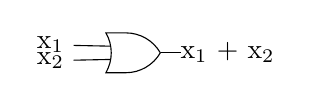
\begin{tikzpicture}
    \node (x) at (0,0.6) {x$_1$};
    \node (y) at (0, 0.4) {x$_2$};
    \node[or gate US, draw, rotate=0, logic gate inputs=nn] at (1, 0.5) (xory) {};
    \draw (x) --(xory.input 1);
    \draw (y) --(xory.input 2);
     \draw (xory.output) --  node[right]{x$_1$ + x$_2$} ($(xory.output) + (0.25, 0)$);

\end{tikzpicture}
\end{document}


